%----------------------------------------------------------------------------------------
%	METODE
%----------------------------------------------------------------------------------------
\section*{HASIL DAN PEMBAHASAN}

\subsection*{Analisis}
Pada penelitian ini, akan dibangun sebuah perangkat lunak untuk membangkitkan kemungkinan jalur dari sebuah program. Jalur-jalur ini dapat dijadikan dasar untuk membangkitkan data uji agar data uji yang digunakan untuk pengujian dapat mewakili semua kemungkinan. Untuk memonitor jalur mana yang dilalui ketika diberikan masukan data uji, maka sistem ini juga akan melakukan penyisipan tag-tag sebagai instrumentasi ke dalam kode program secara otomatis.
Sebelumnya sudah terdapat beberapa program yang dapat membangkitkan CFG seperti Eclipse tetapi library tersebut hanya dapat digunakan di eclipse dan hanya membangkitkan CFG dari kode program java. 
Data yang digunakan dalam penelitian ini didapatkan dari penelitian yang dilakukan oleh \citeauthor{HERMADI2015} (\cite*{HERMADI2015}). Terdapat 15 contoh program yang akan digunakan pada penelitian ini dengan tingkat kompleksitas yang beragam. Contoh program yang akan digunakan dapat dilihat pada Tabel 1.
 \ref{tab:jadwal}.
 
 \begin{table*}[h!]
 	\begin{center}
 		\caption{Contoh program uji}
 		\label{tab:jadwal}
 		\footnotesize
 			\begin{tabular}{|l|l|l|p{9cm}|}
 				\hline
 				\rowcolor[HTML]{EFEFEF} 
 				\multicolumn{1}{|c|}{\cellcolor[HTML]{EFEFEF}\textbf{No}} & \multicolumn{1}{c|}{\cellcolor[HTML]{EFEFEF}\textbf{Program Uji}} & \multicolumn{1}{c|}{\cellcolor[HTML]{EFEFEF}\textbf{Nama}} & \multicolumn{1}{c|}{\cellcolor[HTML]{EFEFEF}\textbf{Deskripsi}}                                                       \\ \hline
 				1                                                         & triangleAhmed2008                                                 & tA2008                                                     & Menentukan tipe dari segitiga apakah termasuk \textit{equilateral}, \textit{isosceles}, \textit{scalene}, atau \textit{not triangle}                      \\ \hline
 				2                                                         & minimaxiAhmed2008                                                 & mmA2008                                                    & Menentukan nilai minimal dan maksimal dari inputan berupa bilangan dalam \textit{array}                                        \\ \hline
 				3                                                         & insertionAhmed2008                                                & iA2008                                                     & Mengurutkan bilangan dalam \textit{array} menggunakan metode \textit{insertion sort}                                                    \\ \hline
 				4                                                         & binnaryAhmed2008                                                  & binA2008                                                   & Mencari indeks sebuah bilangan dalam \textit{array} dengan mengembalikan indeks jika ditemukan dan tidak jika tidak ditemukan. \\ \hline
 				5                                                         & bubbleAhmed2008                                                   & bubA2008                                                   & Mengurutkan bilangan dalam \textit{array} menggunakan metode \textit{bubble sort  }                                                     \\ \hline
 				6                                                         & gcdAhmed2008                                                      & gA2008                                                     & Menghitung GCD atau pembagi dua bilangan terbesar                                                                     \\ \hline
 				7                                                         & remainderAhmed2008                                                & rA2008                                                     & Menghitung sisa hasil bagi                                                                                            \\ \hline
 				8                                                         & mmTriangleAhmed2008                                               & mtA2008                                                    & Program buatan dengan menggabungkan fungsi tA2008 dan mmA2008                                                         \\ \hline
 				9                                                         & triangleMansour2004                                               & tM2004                                                     & Menentukan tipe dari segitiga apakah termasuk \textit{scalene}, \textit{isosceles}, \textit{right}, \textit{iso-right}, \textit{equilateral}                       \\ \hline
 				10                                                        & expintBueno2002                                                   & eB2002                                                     & Fungsi exponensial yang dapat memproses bilangan \textit{integer} dan \textit{float}                                                    \\ \hline
 				11                                                        & quotientBueno2002                                                 & qB2002                                                     & Menghitung hasil bagi dan sisa hasil bagi dari dua buah bilangan bulat positif                                        \\ \hline
 				12                                                        & floatcompBueno2002                                                & fcB2002                                                    & Perbandingan dari tiga buah bilangan float                                                                            \\ \hline
 				13                                                        & findBueno2002                                                     & fB2002                                                     & Mengurutkan bilangan dalam \textit{array} sebagian                                                                             \\ \hline
 				14                                                        & bubbleGong2011                                                    & bG2011                                                     & Mengurutkan bilangan dalam \textit{array} menggunakan metode \textit{bubble sort   }                                                    \\ \hline
 				15                                                        & fitnessMiniMaxiHermadi2014                                        & fmH2014                                                    & Menghitung fungsi \textit{fitness } dari fungsi minimaxiAhmed2008                                                               \\ \hline
 			\end{tabular}
 		\normalsize
 	\end{center}
 \end{table*}

\subsection*{Perancangan}

\subsubsection*{Perancangan \textit{Class Diagram}}
Class diagram dibangun untuk menggambarkan struktur sistem dari segi pendefinisian class-class. Perancangan Class diagram dapat dilihat pada Gambar \ref{fig:classdiagram}.
\begin{figure}[h!]
	\centering
	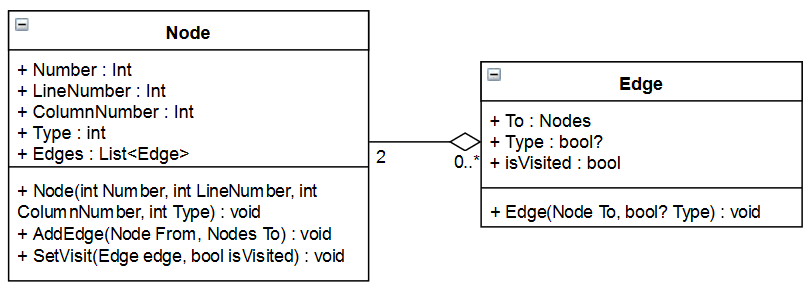
\includegraphics[width=230pt]{gambar/classdiagram}
	\caption{\textit{Class Diagram}}
	\label{fig:classdiagram}
\end{figure}
\subsubsection*{Perancangan Antarmuka}
Perancangan antarmuka meliputi perancangan antarmuka form untuk pengguna memasukkan kode program yang akan di proses dan antarmuka hasil dari proses yang telah dilakukan. Perancangan antarmuka hasil dari proses yang telah dilakukan dapat dilihat pada Gambar \ref{fig:perancanganantarmuka}.
\begin{figure}[h!]
	\centering
	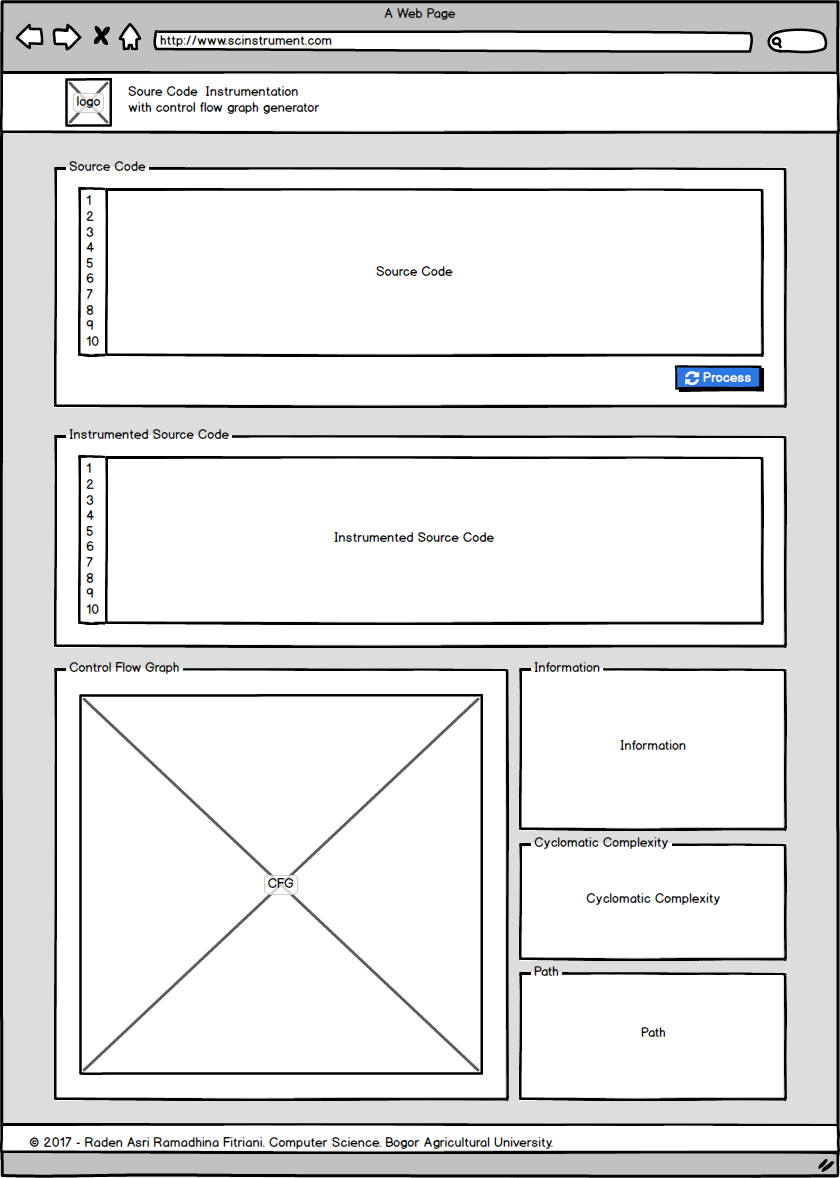
\includegraphics[width=230pt]{gambar/perancanganantarmuka}
	\caption{\textit{Percangan antarmuka sistem}}
	\label{fig:perancanganantarmuka}
\end{figure}

\subsection*{Implementasi}

Aplikasi dibangun dengan menggunakan bahasa pemrograman C\# dan menggunakan IDE Microsoft Visual Studio Ultimate 2013. 
Sebagai contoh, kode program yang digunakan adalah tA2008. Pada kode tA2008 terdapat perintah IF-THEN-ELSE bersarang sebanyak tiga tingkat. 

\subsubsection*{Kode Program}
Gambar \ref{fig:tA2008} merupakan kode program tA2008, yaitu untuk mencari jenis dari segitiga jika diketahui panjang dari setiap sisinya.
\begin{figure}[h!]
	\centering
	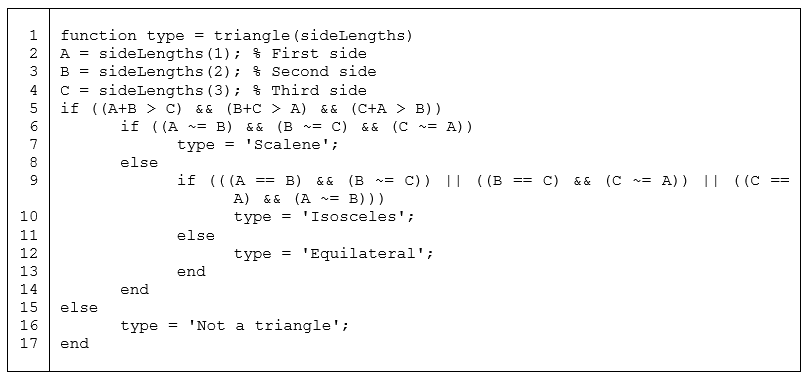
\includegraphics[width=230pt]{gambar/tA2008}
	\caption{\textit{Kode program tA2008}}
	\label{fig:tA2008}
\end{figure}

\subsubsection*{Mengurai Kode Progam ke Format XML}
Penguraian kode program matlab dilakukan dengan menggunakan library  MATLAB-PARSER. Ketika terdapat kesalahan pada kode program, library  ini akan mengembalikan pesan error. Lalu kode program tersebut diurai menjadi file dengan format XML menggunakan library MATLAB-PARSER yang dibuat oleh Suffos (2015). 
Extensible Markup Language (XML) adalah bahasa yang dapat mendeskripsikan sebuah dokumen. XML memiliki banyak bagian yang tidak memiliki struktur yang pasti. XML terdiri atas dua bagian utama, yaitu elemen dan atribut. Elemen yang dapat disebut sebagai node merupakan bagian penting yang dapat menggambarkan struktur dari XML. Sedangkan atribut merupakan bagian yang dapat digunakan sebegai informasi tambahan dari setiap elemen (Hartwell 2017). 

\subsubsection*{Membangkitkan \textit{Graph}}
Setiap dalam tag file XML tersebut akan ditelusuri satu persatu yang termasuk struktur kontrol di dalam bahasa matlab. Sehingga terbentuklah sebuah objek graph yang terdiri dari sekumpulan node dan edge. 
Salah satu cara untuk membaca dan menulis dokumen XML pada framework .NET dan C\# yaitu dengan menggunakan kelas XMLDocument yang terdapat dalam namespace System.XML. Setiap elemen XML yang merupakan struktur kontrol pada program akan menjadi nodes baru di dalam kelas graph. Setiap node berisi informasi nomor baris dan kolom yang akan digunakan untuk melakukan instrumentasi.


\subsubsection*{Membangkitkan Jalur}
\textit{Basis path testing} merupakan salah satu metode pengujian struktural yang menggunakan \textit{source code} dari program untuk menemukan semua jalur yang mungkin dapat dilalui program dan dapat digunakan untuk merancang data uji. Metode ini memastikan semua kemungkinan jalur dijalankan setidaknya satu kali (\cite{BASU2015}). Metode ini terbagi menjadi 4 tahapan, yaitu:
\begin{enumerate}[noitemsep] 
	\item Menggambarkan jalur dalam bentuk \textit{ Control Flow Graph} (CFG)
	\item Menghitung \textit{cyclomatic complexity}
	\item Memilih satu set jalur dasar
	\item Membangkitkan data uji untuk setiap jalur dasar
\end{enumerate}

\subsubsection*{Menghitung \textit{Cyclometic Complexity}}

\textit{Cyclomatic complexity} merupakan suatu sistem pengukuran yang ditemukan oleh \citeauthor{MCCABE} untuk menentukan banyaknya \textit{independent path} dan menunjukan tingkat kompleksitas dari suatu program. \textit{Independent path} adalah jalur yang melintas dalam program yang sekurang-kurangnya terdapat kondisi baru. Perhitungan \textit{Cyclomatic Complexity} dapat dilihat pada persamaan berikut:
\[V(G)=E-N+2\]

Dimana, E menunjukkan jumlah \textit{edges} dan N menunjukkan jumlah \textit{nodes}.

\subsubsection*{Transformasi ke Dalam Format Bahasa Dot}
Graph yang sudah terbentuk akan ditransformasikan ke dalam bentuk format bahasa permrograman dot. Bahasa dot adalah bahasa yang digunakan untuk mengambar graph berarah. Bahasa ini dapat mendeskripsikan 3 macam objek, yaitu graph, nodes, dan edges (Ganser et all 2015).

\subsubsection*{Memvisualisasi \textit{Graph} dalam bentuk CFG}
\textit{Control Flow Graph }(CFG) adalah graph berarah yang merepresentasikan aliran dari sebuah program. Setiap CFG terdiri dari \textit{nodes} dan \textit{edges}. \textit{Nodes} merepresentasikan \textit{statement} atau \textit{expressions}. Sedangkan \textit{edges} merepresentasikan transfer kontrol antar \textit{nodes} (\cite{MCCABE}). Notasi dari CFG dapat dilihat pada Gambar \ref{fig:cfg}.
\begin{figure}[h]
	\centering
	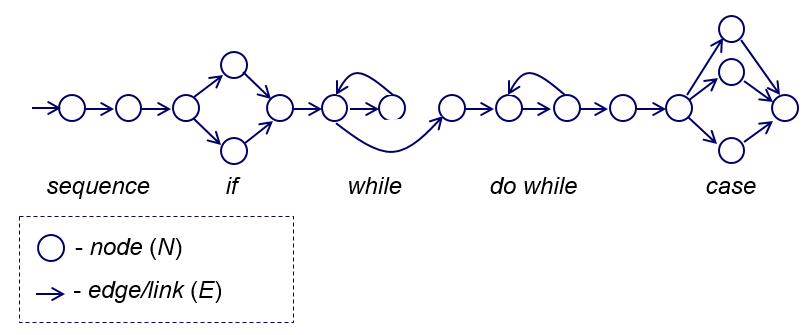
\includegraphics[width=220pt]{gambar/CFG2}
	\caption{Notasi Control Flow Graph (CFG)}
	\label{fig:cfg}
\end{figure}
Setelah file dengan format bahasa dot terbentuk, CFG akan divisualisasikan dengan menggunakan library Graphviz. Graphviz merupakan perangkat lunak open source untuk visualisasi grafik. 

\subsubsection*{Instrumentasi}
Setelah jalur terbentuk, dilakukan juga proses instrumentasi. Instrumentasi merupakan sebuah proses menyisipkan sebuah penanda (tag) di awal atau di akhir setiap blok kode seperti awal setiap perintah, sebelum atau sesudah kondisi terpenuhi atau tidak. Dalam pengujian path testing, penanda ini dapat digunakan untuk memonitor jalur yang dilalui program ketika dijalankan dengan masukan data uji tertentu (Arkeman et al. 2014). 
Instrumentasi dilakukan dengan cara menambahkan dulu variable keluaran bernama traversedPath. Variable in digunakan untuk menyimpan informasi node mana saja yang dilalui ketika diberikan inputan dengan nilai tertentu. Lalu setiap sebelum dan sesudah node percabangan, dilakukan penyisipan kode program berupa perintah untuk memasukkan nilai node yang dilalui. Sehingga ketika program tersebut dijalankan, akan menghasilkan keluaran tambahan bernama traversedPath. 

\subsection*{Testing}

Tahapan ini adalah melakukan evaluasi dari tahapan implementasi. Evaluasi dilakukan dengan membandingkan hasil yang dikeluarkan oleh sistem dengan pembangkitan secara manual dari segi waktu eksekusi. 
